\documentclass{article}
\usepackage{graphicx}
\usepackage[polish]{babel}
\usepackage[T1]{fontenc}
\usepackage{float}
\usepackage[utf8]{inputenc}
\usepackage{csquotes}
\usepackage{amsmath}
\usepackage{array}
\usepackage{biblatex}
\addbibresource{references.bib}

\title{Sprawozdanie AiZSD}
\author{Jan Banot - grupa 2}
\date{01.12.2024}

\begin{document}

\maketitle

\begin{center}
    \textbf{Zadanie 51 - Odległość edycyjna pomiędzy łańcuchami}
\end{center}

\section{Treść zadania}
\begin{figure}[H]
    \centering
    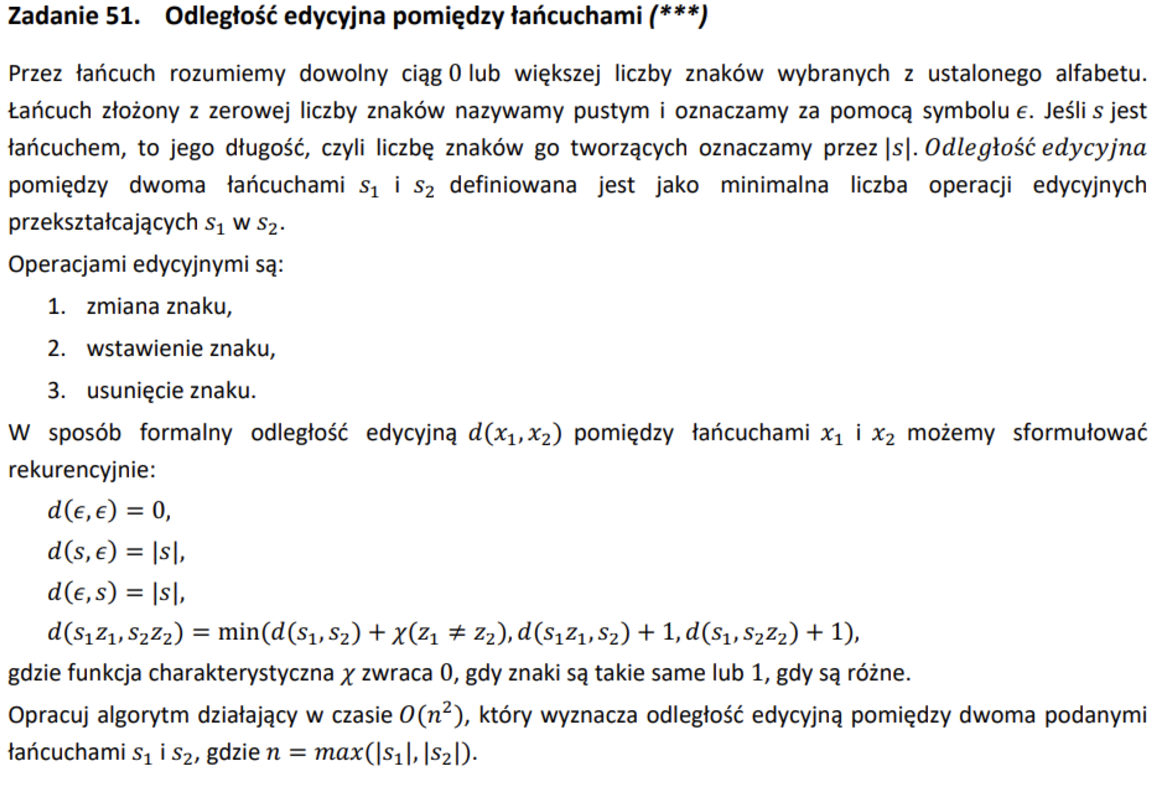
\includegraphics[width=\textwidth]{zadanie51.png}
    \caption{Treść zadania}
    \label{fig:sample}
\end{figure}

\section{Teoria}
\subsection{Opis Problemu}
Odległość edycyjna, znana także jako odległość Levenshteina, to popularna metoda do analizy i korekty tekstu, opracowana przez Vladimira Levenshteina w 1965 roku\cite{levenshtein1966}. Jest to uogólnienie odległości Hamminga, która mierzy odmienność między dwoma skończonymi ciągami znaków.

\vspace{1em}

Odległość ta jest zdefiniowana jako minimalna liczba prostych operacji potrzebnych do przekształcenia jednego ciągu w drugi. Dozwolone operacje to:

\begin{itemize}
    \item Zamiana znaku - zmiana jednego znaku na inny.
    \item Usunięcie znaku - usunięcie jednego znaku z ciągu.
    \item Dodanie znaku - wstawienie nowego znaku do ciągu.
\end{itemize}

\vspace{1em}

Każda z tych operacji ma taką samą wagę. Odległość Levenshteina jest miarą metryczną, co oznacza, że spełnia warunki metryki w przestrzeni ciągów znaków. Znajduje zastosowanie w różnych dziedzinach, takich jak rozpoznawanie mowy, analiza DNA, systemy antyplagiatowe i korekta pisowni.

\subsection{Rekurencyjna definicja}
Odległość Levenshteina można sformułować rekurencyjnie. Rekurencyjna definicja odległości edycyjnej \(d(x_1, x_2)\) między łańcuchami \(x_1\) i \(x_2\) jest następująca:

\vspace{1em}

Warunki brzegowe:
\begin{itemize}
    \item \(d(\epsilon, \epsilon) = 0\): Przekształcenie pustego łańcucha w pusty nie wymaga operacji.
    \item \(d(s, \epsilon) = |s|\): Przekształcenie łańcucha \(s\) w pusty wymaga usunięcia wszystkich znaków.
    \item \(d(\epsilon, s) = |s|\): Przekształcenie pustego łańcucha w \(s\) wymaga wstawienia wszystkich znaków.
\end{itemize}

Definicja rekurencyjna:
\[
    d(s_1z_1, s_2z_2) = \min 
    \begin{cases} 
        d(s_1, s_2) + \chi(z_1 \neq z_2), & \text{(zamiana)} \\ 
        d(s_1z_1, s_2) + 1, & \text{(usunięcie)} \\ 
        d(s_1, s_2z_2) + 1, & \text{(wstawienie)} 
    \end{cases}
\]
, gdzie \(\chi(z_1 \neq z_2)\) wynosi 0, jeśli znaki są takie same, i 1, jeśli są różne.

\section{Rozwiązanie}
\subsection{Struktura optymalnego rozwiązania}
Dzięki tej strukturze możemy efektywnie zastosować programowanie dynamiczne, co pozwala na systematyczne wypełnianie macierzy kosztów i uzyskanie optymalnego rozwiązania.

\subsubsection{Podział na podproblemy}
Odległość edycyjna między dwoma łańcuchami \(s_1\) i \(s_2\) może być rozbita na mniejsze podproblemy, takie jak odległość między prefiksami tych łańcuchów. Każdy podproblem polega na obliczeniu odległości edycyjnej między prefiksami \(s_1[0..i]\) i \(s_2[0..j]\).

\subsubsection{Optymalność podproblemów}
Każde optymalne rozwiązanie dla całego problemu składa się z optymalnych rozwiązań jego podproblemów. Oznacza to, że jeśli znamy minimalną liczbę operacji potrzebnych do przekształcenia prefiksów \(s_1[0..i-1]\) i \(s_2[0..j-1]\), możemy wykorzystać tę wiedzę do obliczenia odległości dla \(s_1[0..i]\) i \(s_2[0..j]\).

\subsubsection{Zależność od trzech operacji}
Optymalne rozwiązanie jest budowane poprzez wybór jednej z trzech operacji: zamiany, usunięcia lub wstawienia, która minimalizuje całkowity koszt. Algorytm dynamiczny wybiera operację, która prowadzi do najmniejszej liczby operacji edycyjnych.

\subsubsection{Przykład}
Rozważmy dwa łańcuchy “kitten” i “sitting”. Optymalne rozwiązanie wymaga minimalnej liczby operacji, które można rozbić na mniejsze kroki, np. “kitten” -> “sitten” -> “sittin” -> “sitting”. Każdy krok opiera się na rozwiązaniu podproblemów dla krótszych prefiksów.

\subsection{Rekurencyjna funkcja kosztu}
\subsubsection{Definicja funkcji}
Niech \(d(i, j)\) oznacza minimalny koszt przekształcenia prefiksu \(s_1[0..i]\) w \(s_2[0..j]\).

\subsubsection{Warunki brzegowe}
\begin{itemize}
    \item \(d(0, 0) = 0\): Przekształcenie pustego łańcucha w pusty nie wymaga operacji.
    \item \(d(i, 0) = i\): Przekształcenie prefiksu \(s_1\) w pusty łańcuch wymaga \(i\) usunięć.
    \item \(d(0, j) = j\): Przekształcenie pustego łańcucha w prefiks \(s_2\) wymaga \(j\) wstawień.
\end{itemize}

\subsubsection{Rekurencyjne wyrażenie}
Dla \(i > 0\) i \(j > 0\):
\[
d(i, j) = \min \begin{cases} 
d(i-1, j) + 1, & \text{(usunięcie)} \\
d(i, j-1) + 1, & \text{(wstawienie)} \\
d(i-1, j-1) + \chi(s_1[i] \neq s_2[j]), & \text{(zamiana)}
\end{cases}
\] 
\label{eq:rekurencyjne-wyrazenie}
Gdzie \(\chi(s_1[i] \neq s_2[j])\) zwraca 0, jeśli znaki są takie same, lub 1, jeśli różne.

\subsubsection{Uzasadnienie}
Funkcja korzysta z wartości już obliczonych dla mniejszych podproblemów, co pozwala na efektywne obliczenie kosztu dla całych łańcuchów. Każda wartość w macierzy jest obliczana na podstawie wcześniej obliczonych wartości, co czyni algorytm efektywnym i pozwala na obliczenie minimalnej liczby operacji edycyjnych.

\subsection{Macierz kosztów}
\subsubsection{Inicjalizacja macierzy}
\begin{enumerate}
    \item Utwórz dwuwymiarową macierz \(D\) o rozmiarze \((m+1) \times (n+1)\), gdzie \(m = |s_1|\) i \(n = |s_2|\).
    \item Zainicjuj pierwszą kolumnę: \(D[i][0] = i\) dla \(0 \leq i \leq m\).
    \item Zainicjuj pierwszy wiersz: \(D[0][j] = j\) dla \(0 \leq j \leq n\).
\end{enumerate}

\subsubsection{Wypełnianie macierzy}
\begin{enumerate}
    \item Iteruj przez wszystkie komórki macierzy, zaczynając od \(i = 1\) i \(j = 1\).
    \item Dla każdej komórki (D[i][j]), oblicz wartość używając rekurencyjnej funkcji kosztu zdefiniowanej w punkcie \ref{eq:rekurencyjne-wyrazenie}.
\end{enumerate}

\subsubsection{Odczytanie wyniku}
Końcowa wartość \(D[m][n]\) zawiera minimalny koszt przekształcenia \(s_1\) w \(s_2\).

\subsubsection{Przykład ilustracyjny}
Rozważmy dwa łańcuchy “kot” i “młot”. Wypełniając macierz, możemy zobaczyć, jak wartości są obliczane krok po kroku. Każda komórka macierzy reprezentuje minimalny koszt przekształcenia odpowiednich prefiksów.

Oto tabela ilustrująca przykład dla wyrazów "kot" i "młot":
\begin{table}[H]
    \centering
    \begin{tabular}{c|c|c|c|c|c}
       &   & \text{m} & \text{\l} & \text{o} & \text{t} \\
    \hline
       & 0 & 1 & 2 & 3 & 4 \\
    \hline
    \text{k} & 1 & 1 & 2 & 3 & 4 \\
    \hline
    \text{o} & 2 & 2 & 2 & 2 & 3 \\
    \hline
    \text{t} & 3 & 3 & 3 & 3 & 2 \\
    \end{tabular}
    \caption{Tabela przedstawiająca minimalny koszt przekształcenia wyrazu "kot" w "młot".}
    \label{tab:kot-mlot}
\end{table}
\begin{itemize}
    \item Inicjalizacja - pierwszy wiersz i kolumna reprezentują przekształcenia pustego łańcucha w prefiksy drugiego łańcucha i odwrotnie.
    \item Obliczenia - każda komórka \(D[i][j]\) jest obliczana na podstawie sąsiednich komórek, zgodnie z rekurencyjną funkcją kosztu.
    \item Wynik końcowy - komórka \(D[3][4]\) (wartość 2) oznacza minimalny koszt przekształcenia "kot" w "młot".
\end{itemize}

\section{Odpowiedź}
\subsection{Algorytm w pseudokodzie}
Poniższy fragment pseudokodu ilustruje, jak algorytm wypełnia macierz kosztów, korzystając z podejścia zstępującego z memoizacją, co pozwala na efektywne obliczanie odległości edycyjnej.

\begin{verbatim}
Funkcja OdległośćEdycyjna(s1, s2):
    Jeśli memo nie istnieje:
        // Struktura do przechowywania wyników podproblemów
        Utwórz pusty memo
    // Klucz identyfikuje unikalny podproblem
    Klucz = (długość(s1), długość(s2))
    Jeśli Klucz jest w memo:
        Zwróć memo[Klucz]
    Jeśli długość(s1) == 0 i długość(s2) == 0:
        // Brak operacji dla pustych łańcuchów
        Zwróć 0
    Jeśli długość(s1) == 0:
        // Wstawienie wszystkich znaków z s2
        Zwróć długość(s2)
    Jeśli długość(s2) == 0:
        // Usunięcie wszystkich znaków z s1
        Zwróć długość(s1)
    s1_prefix = s1 bez ostatniego znaku
    s2_prefix = s2 bez ostatniego znaku
    z1 = ostatni znak s1
    z2 = ostatni znak s2
    koszt_zamiany = 0 jeśli z1 == z2, w przeciwnym razie 1
    Wynik = min(
        // Zamiana
        OdległośćEdycyjna(s1_prefix, s2_prefix) + koszt_zamiany,
        // Wstawienie
        OdległośćEdycyjna(s1, s2_prefix) + 1,
        // Usunięcie
        OdległośćEdycyjna(s1_prefix, s2) + 1
    )
    memo[Klucz] = Wynik
    
    Zwróć Wynik  
\end{verbatim}

\subsection{Analiza złożoności}
\begin{itemize}
    \item Złożoność obliczeniowa - dzięki memoizacji, złożoność czasowa wynosi \(O(m \times n)\), gdzie \(m\) i \(n\) to długości porównywanych łańcuchów. Każdy podproblem jest rozwiązywany tylko raz.
    \item Złożoność pamięciowa - pamięć potrzebna do wykonania procesu memoizacji to również \(O(m \times n)\), ponieważ przechowujemy pośrednie wyniki dla wszystkich możliwych podproblemów.
\end{itemize}

\subsection{Implementacja rozwiązania w języku Python}
Poniżej znajduje się implementacja algorytmu obliczającego odległość edycyjną z wykorzystaniem memoizacji. Podejście to pozwala na efektywne obliczanie minimalnej liczby operacji potrzebnych do przekształcenia jednego łańcucha w drugi, unikając wielokrotnego rozwiązywania tych samych podproblemów.

\begin{verbatim}
def edit_distance(s1, s2, memo=None):
    if memo is None:
        memo = {}
    
    key = (len(s1), len(s2))
    # If result already calculated, return it
    if key in memo:
        return memo[key]
        
    # Base cases
    if len(s1) == 0:
        return len(s2)
    if len(s2) == 0:
        return len(s1)
        
    # Get prefixes and last characters
    s1_prefix = s1[:-1]
    s2_prefix = s2[:-1]
    z1 = s1[-1]
    z2 = s2[-1]

    # Calculate replacement cos
    rep_cost = 0 if z1 == z2 else 1
    
    result = min(
        edit_distance(s1_prefix, s2_prefix, memo) + repl_cost,
        edit_distance(s1, s2_prefix, memo) + 1,
        edit_distance(s1_prefix, s2, memo) + 1,
    )
    
    memo[key] = result
    return result
\end{verbatim}

\printbibliography

\end{document}